% !TEX TS-program = pdflatex
% !TEX encoding = UTF-8 Unicode

% This is a simple template for a LaTeX document using the "article" class.
% See "book", "report", "letter" for other types of document.

\documentclass[11pt]{article} % use larger type; default would be 10pt

\usepackage[utf8]{inputenc} % set input encoding (not needed with XeLaTeX)
\usepackage{alltt}
\usepackage{graphicx}

%%% Examples of Article customizations
% These packages are optional, depending whether you want the features they provide.
% See the LaTeX Companion or other references for full information.

%%% PAGE DIMENSIONS
\usepackage{geometry} % to change the page dimensions
\geometry{a4paper} % or letterpaper (US) or a5paper or....
% \geometry{margin=2in} % for example, change the margins to 2 inches all round
% \geometry{landscape} % set up the page for landscape
%   read geometry.pdf for detailed page layout information

\usepackage{graphicx} % support the \includegraphics command and options

% \usepackage[parfill]{parskip} % Activate to begin paragraphs with an empty line rather than an indent

%%% PACKAGES
\usepackage{booktabs} % for much better looking tables
\usepackage{array} % for better arrays (eg matrices) in maths
\usepackage{paralist} % very flexible & customisable lists (eg. enumerate/itemize, etc.)
\usepackage{verbatim} % adds environment for commenting out blocks of text & for better verbatim
\usepackage{subfig} % make it possible to include more than one captioned figure/table in a single float
\usepackage{amsmath}
% These packages are all incorporated in the memoir class to one degree or another...

%%% HEADERS & FOOTERS
\usepackage{fancyhdr} % This should be set AFTER setting up the page geometry
\pagestyle{fancy} % options: empty , plain , fancy
\renewcommand{\headrulewidth}{0pt} % customise the layout...
\lhead{}\chead{}\rhead{}
\lfoot{}\cfoot{\thepage}\rfoot{}

%%% SECTION TITLE APPEARANCE
\usepackage{sectsty}
\allsectionsfont{\sffamily\mdseries\upshape} % (See the fntguide.pdf for font help)
% (This matches ConTeXt defaults)

%%% ToC (table of contents) APPEARANCE
\usepackage[nottoc,notlof,notlot]{tocbibind} % Put the bibliography in the ToC
\usepackage[titles,subfigure]{tocloft} % Alter the style of the Table of Contents
\renewcommand{\cftsecfont}{\rmfamily\mdseries\upshape}
\renewcommand{\cftsecpagefont}{\rmfamily\mdseries\upshape} % No bold!



\title{Numerical Analysis Homework 1}
\author{Margaret Dorsey}
%\date{} % Activate to display a given date or no date (if empty),
         % otherwise the current date is printed 

\begin{document}
\maketitle

\section*{Problems 1 and 2}
\par Problems 1 and 2 can be found as problem1.c / problem1.exe and problem2.c / problem2.exe.

\section*{Problem 3}
\subsection*{Raw Output}
\begin{alltt}
Please enter the dimension of the matrix: 4
Enter your values, row major: 
2.000000
3.000000
1.000000
5.000000
1.000000
0.000000
3.000000
1.000000
0.000000
2.000000
-3.000000
2.000000
0.000000
2.000000
3.000000
1.000000

18.000000
-35.000000
-28.000000
1.000000
9.000000
-18.000000
-14.000000
1.000000
-2.000000
4.000000
3.000000
0.000000
-12.000000
24.000000
19.000000
-1.000000
\end{alltt}
\subsection*{Matrix Form}
\[
\begin{bmatrix}
2&3&1&5\\
1&0&3&1\\
0&2&-3&2 \\
0&2&3&1
\end{bmatrix}
^{-1}
=
\begin{bmatrix}
18&-35&-28&1\\
9&-18&-14&1\\
-2&4&3&0 \\
-12&24&19&-1
\end{bmatrix}
\]

\section*{Problem 4}
\begin{enumerate}[a.)]
\item $10.5d = 1010.1b = 01000000001001010\ldots0$
\par $10d = 1010d, .5d * 2d = 1.0d = 1.0b = .1b * 2b$. So $(10+.5)d = (1010 + .1)b$.
\par $1010.1 = 1.0101 x 2^3 = 1.0101 \times 2^{1026 - 1023}$
\item $\frac{1}{3}d = \overline{.01}b = 001111111101010101\ldots01$
\par $\frac{1}{3} * 2 = \frac{2}{3}$, $\frac{2}{3} * 2 = 1 + \frac{1}{3} \rightarrow \frac{1}{3} * 2 = \ldots = \overline{.01}b$
\par $\overline{.01} = 1.\overline{01} x 2^{-2} = 1.\overline{01} \times 2^{1021 - 1023}$
\item $\frac{22}{7}d = 11.\overline{001}b = 010000000000100100100\ldots001$
\par $\frac{22}{7} = 3 + \frac{1}{7} \rightarrow \frac{1}{7} * 2 = \frac{2}{7} \rightarrow \frac{4}{7} \rightarrow 1 + {1}{7} \ldots = (11.\overline{001})b$
\par $11.\overline{001} = 1.1\overline{001} \times 2 = 1001001 \ldots 001$
\end{enumerate}

\section*{Problem 5}

\subsection*{Bisection}
\subsubsection*{Raw Output}
\begin{alltt}
i: 0	a: 1.000000000	b: 2.000000000	value: -1.000000000 
i: 1	a: 1.000000000	b: 1.500000000	value: 1.375000000 
i: 2	a: 1.250000000	b: 1.500000000	value: -0.046875000 
i: 3	a: 1.250000000	b: 1.375000000	value: 0.599609375 
i: 4	a: 1.250000000	b: 1.312500000	value: 0.260986328 
i: 5	a: 1.250000000	b: 1.281250000	value: 0.103302002 
i: 6	a: 1.250000000	b: 1.265625000	value: 0.027286530 
i: 7	a: 1.257812500	b: 1.265625000	value: -0.010024548 
i: 8	a: 1.257812500	b: 1.261718750	value: 0.008573234 
i: 9	a: 1.259765625	b: 1.261718750	value: -0.000740074 
i: 10	a: 1.259765625	b: 1.260742188	value: 0.003912973 
i: 11	a: 1.259765625	b: 1.260253906	value: 0.001585548 
i: 12	a: 1.259765625	b: 1.260009766	value: 0.000422512 
i: 13	a: 1.259887695	b: 1.260009766	value: -0.000158837 
i: 14	a: 1.259887695	b: 1.259948730	value: 0.000131823 
i: 15	a: 1.259918213	b: 1.259948730	value: -0.000013510 
i: 16	a: 1.259918213	b: 1.259933472	value: 0.000059156 
i: 17	a: 1.259918213	b: 1.259925842	value: 0.000022822 
i: 18	a: 1.259918213	b: 1.259922028	value: 0.000004656 
i: 19	a: 1.259920120	b: 1.259922028	value: -0.000004427 
i: 20	a: 1.259920120	b: 1.259921074	value: 0.000000114 
i: 21	a: 1.259920597	b: 1.259921074	value: -0.000002156 
i: 22	a: 1.259920835	b: 1.259921074	value: -0.000001021 
i: 23	a: 1.259920955	b: 1.259921074	value: -0.000000453 
i: 24	a: 1.259921014	b: 1.259921074	value: -0.000000169 
i: 25	a: 1.259921044	b: 1.259921074	value: -0.000000028 
i: 26	a: 1.259921044	b: 1.259921059	value: 0.000000043 
i: 27	a: 1.259921044	b: 1.259921052	value: 0.000000008 
i: 28	a: 1.259921048	b: 1.259921052	value: -0.000000010 
i: 29	a: 1.259921050	b: 1.259921052	value: -0.000000001 
\end{alltt}

\subsubsection*{Analysis}
The bisection method took 29 iterations to successfully find the root within an error of $10^{-8}$,  which agrees with the error formula for bisection method, $n \geq \frac{\log(2) - \log(10^{-8})}{\log 2} \approx  28$.  The method converges slowly, but very consistently, as expected.
\subsection*{Secant}
\subsubsection*{Raw Output}
\begin{verbatim}
i: 0	a: 2.000000000	b: 0.500000000	value: -1.875000000
i: 1	a: 0.500000000	b: 0.857142857	value: -1.370262391
i: 2	a: 0.857142857	b: 1.826714801	value: 4.095540811
i: 3	a: 1.826714801	b: 1.100211976	value: -0.668230377
i: 4	a: 1.100211976	b: 1.202120997	value: -0.262821088
i: 5	a: 1.202120997	b: 1.268187169	value: 0.039623768
i: 6	a: 1.268187169	b: 1.259531737	value: -0.001853412
i: 7	a: 1.259531737	b: 1.259918506	value: -0.000012113
i: 8	a: 1.259918506	b: 1.259921051	value: 0.000000004
i: 9	a: 1.259921051	b: 1.259921050	value: -0.000000000
\end{verbatim}

\subsubsection*{Analysis}
The secant method took only 9 iterations to successfully find the root within 8 digits of accuracy,
which considering the method is superlinearly convergent when appropriate initial values are 
chosen, it is not surprising that it was the the second fastest method to converge.
\subsection*{False Position}
\subsubsection*{Raw Output}
\begin{verbatim}
i: 0	a: 0.500000000	b: 2.000000000	value: -1.875000000
i: 1	a: 0.857142857	b: 2.000000000	value: -1.370262391
i: 2	a: 1.069620253	b: 2.000000000	value: -0.776260854
i: 3	a: 1.176200769	b: 2.000000000	value: -0.372787106
i: 4	a: 1.224390317	b: 2.000000000	value: -0.164477725
i: 5	a: 1.245084774	b: 2.000000000	value: -0.069824644
i: 6	a: 1.253768993	b: 2.000000000	value: -0.029154523
i: 7	a: 1.257377460	b: 2.000000000	value: -0.012088652
i: 8	a: 1.258870669	b: 2.000000000	value: -0.004997956
i: 9	a: 1.259487511	b: 2.000000000	value: -0.002063890
i: 10	a: 1.259742146	b: 2.000000000	value: -0.000851855
i: 11	a: 1.259847230	b: 2.000000000	value: -0.000351525
i: 12	a: 1.259890591	b: 2.000000000	value: -0.000145047
i: 13	a: 1.259908483	b: 2.000000000	value: -0.000059848
i: 14	a: 1.259915865	b: 2.000000000	value: -0.000024693
i: 15	a: 1.259918910	b: 2.000000000	value: -0.000010189
i: 16	a: 1.259920167	b: 2.000000000	value: -0.000004204
i: 17	a: 1.259920686	b: 2.000000000	value: -0.000001734
i: 18	a: 1.259920900	b: 2.000000000	value: -0.000000716
i: 19	a: 1.259920988	b: 2.000000000	value: -0.000000295
i: 20	a: 1.259921024	b: 2.000000000	value: -0.000000122
i: 21	a: 1.259921039	b: 2.000000000	value: -0.000000050
i: 22	a: 1.259921046	b: 2.000000000	value: -0.000000021
i: 23	a: 1.259921048	b: 2.000000000	value: -0.000000009
i: 24	a: 1.259921049	b: 2.000000000	value: -0.000000004
i: 25	a: 1.259921050	b: 2.000000000	value: -0.000000001
i: 26	a: 1.259921050	b: 2.000000000	value: -0.000000001
\end{verbatim}
\subsubsection*{Analysis}
False position performed almost as poorly as bisection method, although the reason for this can be easily seen in the output - the right endpoint remains at the initial value for every iteration to maintain bracketing, which stunts it significantly compared to its' sibling, the secant method. 
\subsection*{FPI}
\begin{enumerate}
\item $g(x) = \frac{x}{2}+ \frac{1}{x^2}$
\subsubsection*{Raw Output}
\begin{verbatim}
i: 0	x: 1.000000000	value: 1.500000000
i: 1	x: 1.500000000	value: 1.194444444
i: 2	x: 1.194444444	value: 1.298141638
i: 3	x: 1.298141638	value: 1.242482157
i: 4	x: 1.242482157	value: 1.269009360
i: 5	x: 1.269009360	value: 1.255474294
i: 6	x: 1.255474294	value: 1.262168081
i: 7	x: 1.262168081	value: 1.258803531
i: 8	x: 1.258803531	value: 1.260481298
i: 9	x: 1.260481298	value: 1.259641299
i: 10	x: 1.259641299	value: 1.260061018
i: 11	x: 1.260061018	value: 1.259851089
i: 12	x: 1.259851089	value: 1.259956036
i: 13	x: 1.259956036	value: 1.259903558
i: 14	x: 1.259903558	value: 1.259929796
i: 15	x: 1.259929796	value: 1.259916677
i: 16	x: 1.259916677	value: 1.259923236
i: 17	x: 1.259923236	value: 1.259919957
i: 18	x: 1.259919957	value: 1.259921597
i: 19	x: 1.259921597	value: 1.259920777
i: 20	x: 1.259920777	value: 1.259921187
i: 21	x: 1.259921187	value: 1.259920982
i: 22	x: 1.259920982	value: 1.259921084
i: 23	x: 1.259921084	value: 1.259921033
i: 24	x: 1.259921033	value: 1.259921058
i: 25	x: 1.259921058	value: 1.259921046
i: 26	x: 1.259921046	value: 1.259921052
i: 27	x: 1.259921052	value: 1.259921049
i: 28	x: 1.259921049	value: 1.259921050
\end{verbatim}
\subsubsection*{Analysis}
This choice of $g(x)$ did converge, but very slowly. This makes intuitive sense, considering that the derivative of $g$, $\frac{1}{2} - \frac{2}{x^3}$, is $-.524$ at $1.25$, near the root.  This is fairly large in absolute value, considering we would like it to be as close to $0$ as possible for fast convergence, and thus our rate of convergence is mediocre at best.
\item $g(x) = \frac{2x}{3}+ \frac{2}{3x^2}$
\subsubsection*{Raw Output}
\begin{verbatim}
i: 0	x: 1.000000000	value: 1.333333333
i: 1	x: 1.333333333	value: 1.263888889
i: 2	x: 1.263888889	value: 1.259933493
i: 3	x: 1.259933493	value: 1.259921050
\end{verbatim}
\subsubsection*{Analysis}
This was by far the fastest convergence of any of the methods, and by examining the value of $g'(x)$ at $1.25$ (near the root), we see why - the value is only $-0.016$, which is relatively close to 0, which would give us quadratic convergence. Thus it managed to outdo even the superlinearly convergent secant method, although it required some lucky choices on our part.
\item $g(x) = x - .25(x^3 - 2)$
\subsubsection*{Raw Output}
\begin{verbatim}
i: 0	x: 1.000000000	value: 1.250000000
i: 1	x: 1.250000000	value: 1.261718750
i: 2	x: 1.261718750	value: 1.259575441
i: 3	x: 1.259575441	value: 1.259986793
i: 4	x: 1.259986793	value: 1.259908518
i: 5	x: 1.259908518	value: 1.259923438
i: 6	x: 1.259923438	value: 1.259920595
i: 7	x: 1.259920595	value: 1.259921137
i: 8	x: 1.259921137	value: 1.259921033
i: 9	x: 1.259921033	value: 1.259921053
i: 10	x: 1.259921053	value: 1.259921049
\end{verbatim}
\subsubsection*{Analysis}
This choice of $g(x)$ was superlinear, comparable to the secant method, but clearly not as good as our second choice of $g$. This is again explained by the absolute value of $g'(x)$ at $1.25$ - a respectable but not particularly small $0.1719$.
\end{enumerate}

\section*{Problem 6}
The functions $g_i(x)$ that I constructed are 
$$g_1(x) = \frac{-1}{14.5}f(x) + x$$
$$g_2(x) = \frac{1}{8}f(x) + x$$
$$g_3(x) = \frac{1}{16}f(x) + x$$
where constants were obtained by taking the negative reciprocal of the approximate derivative of $f(x) = 2x^3 - 8x -1$ at
the roots.
\subsection*{Root 1: $x  \approx -1.9343$ }
\subsubsection*{Raw Output - Initial Guess -2}
 
\begin{alltt}

--------------------------
 FALSE POSITION METHOD G_1
 -----------------------


i: 0	x: -2.000000000	value: -1.931034483
i: 1	x: -1.931034483	value: -1.934277890
i: 2	x: -1.934277890	value: -1.934297805
i: 3	x: -1.934297805	value: -1.934297876


--------------------------
 FALSE POSITION METHOD G_2
 -----------------------


i: 0	x: -2.000000000	value: -2.125000000
i: 1	x: -2.125000000	value: -2.523925781
i: 2	x: -2.523925781	value: -4.144478854
i: 3	x: -4.144478854	value: -17.922122637
i: 4	x: -17.922122637	value: -1439.282558733
i: 5	x: -1439.282558733	value: -745380791.274546146
i: 6	x: -745380791.274546146	value: -103531998791534679437606912.00
\vdots
i: 9	x:-5338649661037961749139249029218884120044021
	   0977416127945813409938556185753597183064238200
	   750388647947661043746914449187671738349912853258
	   84453612284250387716704357639249146159480027431914962
	   774780796808037723725177713273312943013888.000000000	
value: -inf

--------------------------
 FALSE POSITION METHOD G_3
 -----------------------


i: 0	x: -2.000000000	value: -2.062500000
i: 1	x: -2.062500000	value: -2.190460205
i: 2	x: -2.190460205	value: -2.471490348
i: 3	x: -2.471490348	value: -3.185309780
i: 4	x: -3.185309780	value: -5.695003010
i: 5	x: -5.695003010	value: -25.998297789
i: 6	x: -25.998297789	value: -2209.630166633
i: 7	x: -2209.630166633	value: -1348556479.545314789
i: 8	x: -1348556479.545314789	value: -306561373512356053857075200.000000000
\vdots
i: 11	x: -5838441740431293736846375112159843378479548958498592641
32671391884041528845831961691936557706785459758584326765673067
51835622705700753107807916490776000946596515913787553257632307
52325937701298656699774349701532742109721820722207129600.000000000	
value: -inf
\end{alltt}
\subsection*{Root 2: $x \approx -0.12549$}
\subsubsection*{Raw Output - Initial Guess 0}
\begin{alltt}
 

--------------------------
 FALSE POSITION METHOD G_1
 -----------------------


i: 0	x: 0.000000000	value: 0.068965517
i: 1	x: 0.068965517	value: 0.175935731
i: 2	x: 0.175935731	value: 0.341218093
i: 3	x: 0.341218093	value: 0.592962151
i: 4	x: 0.592962151	value: 0.960322243
i: 5	x: 0.960322243	value: 1.436965242
i: 6	x: 1.436965242	value: 1.889477770
i: 7	x: 1.889477770	value: 2.070475964
i: 8	x: 2.070475964	value: 2.057516112
i: 9	x: 2.057516112	value: 2.060251590
i: 10	x: 2.060251590	value: 2.059698076
i: 11	x: 2.059698076	value: 2.059811107
i: 12	x: 2.059811107	value: 2.059788068
i: 13	x: 2.059788068	value: 2.059792766
i: 14	x: 2.059792766	value: 2.059791808
i: 15	x: 2.059791808	value: 2.059792003
i: 16	x: 2.059792003	value: 2.059791963
i: 17	x: 2.059791963	value: 2.059791971
i: 18	x: 2.059791971	value: 2.059791970


--------------------------
 FALSE POSITION METHOD G_2
 -----------------------


i: 0	x: 0.000000000	value: -0.125000000
i: 1	x: -0.125000000	value: -0.125488281
i: 2	x: -0.125488281	value: -0.125494026
i: 3	x: -0.125494026	value: -0.125494094


--------------------------
 FALSE POSITION METHOD G_3
 -----------------------


i: 0	x: 0.000000000	value: -0.062500000
i: 1	x: -0.062500000	value: -0.093780518
i: 2	x: -0.093780518	value: -0.109493356
i: 3	x: -0.109493356	value: -0.117410765
\vdots
i: 22	x: -0.125494056	value: -0.125494075
i: 23	x: -0.125494075	value: -0.125494085
i: 24	x: -0.125494085	value: -0.125494089
i: 25	x: -0.125494089	value: -0.125494092
i: 26	x: -0.125494092	value: -0.125494093

\end{alltt}
\subsection*{Root 3: $x \approx 2.0598$}
\subsubsection*{Raw Output - Initial Guess 2}
\begin{alltt}
 

--------------------------
 FALSE POSITION METHOD G_1
 -----------------------


i: 0	x: 2.000000000	value: 2.068965517
i: 1	x: 2.068965517	value: 2.057849709
i: 2	x: 2.057849709	value: 2.060184771
i: 3	x: 2.060184771	value: 2.059711749
i: 4	x: 2.059711749	value: 2.059808321
i: 5	x: 2.059808321	value: 2.059788636
i: 6	x: 2.059788636	value: 2.059792650
i: 7	x: 2.059792650	value: 2.059791831
i: 8	x: 2.059791831	value: 2.059791998
i: 9	x: 2.059791998	value: 2.059791964
i: 10	x: 2.059791964	value: 2.059791971
i: 11	x: 2.059791971	value: 2.059791970


--------------------------
 FALSE POSITION METHOD G_2
 -----------------------


i: 0	x: 2.000000000	value: 1.875000000
i: 1	x: 1.875000000	value: 1.522949219
i: 2	x: 1.522949219	value: 0.758072328
i: 3	x: 0.758072328	value: -0.016088951
i: 4	x: -0.016088951	value: -0.125001041
i: 5	x: -0.125001041	value: -0.125488293
i: 6	x: -0.125488293	value: -0.125494026
i: 7	x: -0.125494026	value: -0.125494094


--------------------------
 FALSE POSITION METHOD G_3
 -----------------------


i: 0	x: 2.000000000	value: 1.937500000
i: 1	x: 1.937500000	value: 1.815399170
i: 2	x: 1.815399170	value: 1.593070099
i: 3	x: 1.593070099	value: 1.239411117
i: 4	x: 1.239411117	value: 0.795194169
i: 5	x: 0.795194169	value: 0.397950600
i: 6	x: 0.397950600	value: 0.144352965
i: 7	x: 0.144352965	value: 0.010052482
\vdots
i: 30	x: -0.125494053	value: -0.125494074
i: 31	x: -0.125494074	value: -0.125494084
i: 32	x: -0.125494084	value: -0.125494089
i: 33	x: -0.125494089	value: -0.125494092
i: 34	x: -0.125494092	value: -0.125494093


\end{alltt}

\subsection*{Analysis}
$g_1(x)$ is surprisingly stable and useful, converging to two different roots, and converging for all 3 initial values. $g_2(x)$ does a good job of finding the second root, although it diverged for initial value $-2$, it converged to the root it was chosen for in both other cases. Perplexingly, $g_3$, while it does sometimes converge, does not seem to converge towards the third root even when nearby, despite being chosen explicitly to find that root. Fortunately, $g_1$ can find the third root, and thus we do have a function $g_i(x)$ for each root, just not as expected.

\par Ultimately, $g_1$ and $g_2$ together form a good pair of functions for finding the roots of this equation - $g_3$ is fairly slow to converge in all cases, and the root that it finds can be found by $g_2$. The functions are all fairly stable considering the usual instability of fixed point iteration, with $g_2$ and $g_3$ both diverging relatively quickly for the negative initial value, but converging eventually otherwise, and $g_1$ converging when started near any of the 3 real roots.
\section*{Problem 7}
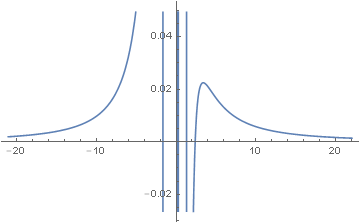
\includegraphics[scale=.5]{problem7plota.png}
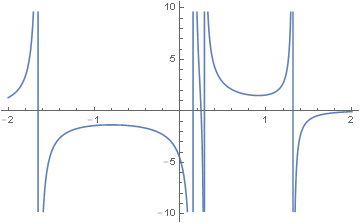
\includegraphics[scale=.5]{problem7plotb.png}
\par Considering the above graphs of the function $\Omega_1 - \Omega_2$, it is not surprising that the secant method fails
miserably. As the method approaches a root, the secant lines can become near vertical, leading to unpredictable results. In addition, the asymptotic behavior at larger values can trick a numerical method into believing it has found a root at very large positive and very large negative values of $x$.
	The simplest solution to the problem is to shrink our bounds until we avoid the asymptotic behavior - for example, bounds of .2 and .25 are sufficient to find the root quickly, and this would be easily found by experimentation by simply trying each .05 length interval in the original interval, even if we didn't  know where the root was exactly.

\subsection*{Raw Output of Secant Method with [-1,1]}
\begin{alltt}
i: 0	a: 1.000000000	b: -0.046482412	value: -3.702651461
i: 1	a: -0.046482412	b: 0.690415093	value: 1.780384308
i: 2	a: 0.690415093	b: 0.451138749	value: 3.331354064
i: 3	a: 0.451138749	b: 0.965084439	value: 1.521238272
i: 4	a: 0.965084439	b: 1.397009213	value: -2.471275853
i: 5	a: 1.397009213	b: 1.129657557	value: 1.966787495
i: 6	a: 1.129657557	b: 1.248138041	value: 4.210222009
i: 7	a: 1.248138041	b: 1.025787382	value: 1.595297137

\vdots
i: 42	a: -3937.724726937	b: -5215.963537543	value: 0.000000028
i: 43	a: -5215.963537543	b: -6909.269396967	value: 0.000000016
i: 44	a: -6909.269396967	b: -9152.422040822	value: 0.000000009
i: 45	a: -9152.422040822	b: -12123.966602370	value: 0.000000005
i: 46	a: -12123.966602370	b: -16060.425023712	value: 0.000000003
i: 47	a: -16060.425023712	b: -21275.122167236	value: 0.000000002
i: 48	a: -21275.122167236	b: -28183.125103398	value: 0.000000001

\end{alltt}
\subsection*{Raw Output of Secant Method with [.2,.25]}
\begin{alltt}

i: 0	a: 0.200000000	b: 0.243206198	value: 0.195326626
i: 1	a: 0.243206198	b: 0.244224922	value: -0.014224914
i: 2	a: 0.244224922	b: 0.244155768	value: 0.000179400
i: 3	a: 0.244155768	b: 0.244156630	value: 0.000000166
i: 4	a: 0.244156630	b: 0.244156630	value: -0.000000000

\end{alltt}
\section*{Problem 8}
\subsection*{Raw Output}
\subsubsection*{First Method}
\begin{alltt}
Enter the x value to approximate at: 2
Actual value: 403.428793492735 
n: 1	value: 1.000000000000
n: 2	value: 7.000000000000
n: 3	value: 25.000000000000
n: 4	value: 61.000000000000
n: 5	value: 115.000000000000

\vdots
n: 25	value: 403.428791117540
n: 26	value: 403.428792950427
n: 27	value: 403.428793373400
\end{alltt}

\begin{alltt}
Enter the x value to approximate at: -2
Actual value: 0.002478752177 
Enter the x value to approximate at: Actual value: 0.002478752177 
n: 1	value: 1.000000000000
n: 2	value: -5.000000000000
n: 3	value: 13.000000000000
n: 4	value: -23.000000000000

\vdots
n: 33	value: 0.002478752181
n: 34	value: 0.002478752176
\end{alltt}

\begin{alltt}
Enter the x value to approximate at: -12
Actual value: 0.000000000000 
n: 1	value: 1.000000000000
n: 2	value: -35.000000000000
n: 3	value: 613.000000000000
\vdots

n: 98	value: -0.058785404183
n: 99	value: -0.023849127767
n: 100	value: -0.036553228282
\end{alltt}

\begin{alltt}
Enter the x value to approximate at: Actual value: 114200738981568423454048256.000000000000 
n: 1	value: 1.000000000000
n: 2	value: 61.000000000000
n: 3	value: 1861.000000000000
n: 4	value: 37861.000000000000
n: 5	value: 577861.000000000000

\vdots
n: 98	value: 114200260606732911767453696.000000000000
n: 99	value: 114200453117080195064397824.000000000000
n: 100	value: 114200569790017939393478656.000000000000

\end{alltt}

\begin{alltt}
Enter the x value to approximate at: -20
Actual value: 0.000000000000 
n: 1	value: 1.000000000000
n: 2	value: -59.000000000000
n: 3	value: 1741.000000000000
n: 4	value: -34259.000000000000
n: 5	value: 505741.000000000000
\vdots

n: 98	value: -119692383293604823040.000000000000
n: 99	value: 72817963995076067328.000000000000
n: 100	value: -43854973755639627776.000000000000
\end{alltt}


\subsubsection*{Second Method}

\begin{alltt}
Enter the x value to approximate at: 2
Actual value: 403.428793492735 
n: 1	value: 1.000000000000
n: 2	value: 7.000000000000
n: 3	value: 25.000000000000
n: 4	value: 61.000000000000
n: 5	value: 115.000000000000
n: 6	value: 179.800000000000
n: 7	value: 244.600000000000
n: 8	value: 300.142857142857

\vdots
n: 32	value: 403.428793492698
n: 33	value: 403.428793492728
n: 34	value: 403.428793492734
n: 35	value: 403.428793492735
n: 36	value: 403.428793492735
n: 37	value: 403.428793492735
\end{alltt}

\begin{alltt}
Enter the x value to approximate at: -2
Actual value: 0.002478752177 
n: 1	value: 1.000000000000
n: 2	value: -5.000000000000
n: 3	value: 13.000000000000
n: 4	value: -23.000000000000
n: 5	value: 31.000000000000
n: 6	value: -33.800000000000

\vdots
n: 37	value: 0.002478752177
n: 38	value: 0.002478752177
n: 39	value: 0.002478752177
\end{alltt}

\begin{alltt}
Enter the x value to approximate at: -12
Actual value: 0.000000000000 
n: 1	value: 1.000000000000
n: 2	value: -35.000000000000
n: 3	value: 613.000000000000
n: 4	value: -7163.000000000000
n: 5	value: 62821.000000000000
n: 6	value: -441063.799999999988

\vdots 
n: 125	 value: -0.033183842925
n: 126	 value: -0.033183842925
n: 127	 value: -0.033183842925

\end{alltt}

\begin{alltt}
Enter the x value to approximate at: 20
Actual value: 114200738981568423454048256.000000000000 
n: 1	value: 1.000000000000
n: 2	value: 61.000000000000
n: 3	value: 1861.000000000000
n: 4	value: 37861.000000000000

\vdots
n: 133	value: 114200738981568389094309888.000000000000
n: 134	value: 114200738981568406274179072.000000000000
n: 135	value: 114200738981568423454048256.000000000000
n: 136	value: 114200738981568423454048256.000000000000

\end{alltt}

\begin{alltt}
Enter the x value to approximate at: Actual value: 0.000000000000 
n: 1	value: 1.000000000000
n: 2	value: -59.000000000000
n: 3	value: 1741.000000000000
n: 4	value: -34259.000000000000

\vdots
n: 174	value: 722745700.930318236351
n: 175	value: 722745700.930318593979
n: 176	value: 722745700.930318474770
n: 177	value: 722745700.930318474770
\end{alltt}

\subsection*{Analysis}
\par For positive $x$ and small (in absolute value) negative $x$, the second method is much more accurate - obviously due to finding the answer to $10^{-15}$ precision instead of a smaller relative precision, and also because it is not constrained to only $100$ iterations. However, for large negative $x$, neither method converges - likely because the series is not absolutely convergent, and the extremely large (in absolute value) terms that appear late in the series overflow even 64 bit floating point numbers. Because the second method is only looking for the distance between sums to become small, this floating point overflow actually leads to an incorrect convergene - the first method simply runs out of iterations before it can return an answer at all.

\section*{Problem 9}

\section*{Problem 10}
\begin{enumerate}[i.)]
\item
\item
\item
\item
\item
\end{enumerate}


\end{document}
